\section{External memory implicit searching}
Given a static input array $A$ of $N$ keys in the EMM (external memory or cache-aware model), describe how to organize the keys inside $A$ by suitably permuting them during a preprocessing step, so that any subequent search of a key requires $O(\log_B N)$ block transfers using just $O(1)$ memory words of auxiliary storage (besides those necessary to store $A$). Clearly, the CPU complexity should remain $O(\log N)$. Discuss the I/O complexity of the above preprocessing, assuming that it can uses $O(N/B)$ blocks of auxiliary storage. (Note that the additional $O(N/B)$ blocks are employed only during the preprocessing; after that, they are discarded as the search is implicit and thus just $O(1)$ words can be employed.)

\vspace{0.5cm}
\paragraph{Solution.} The idea is to construct a B-tree, a balanced search tree where each node has $B$ keys. The keys inside a node $x$ divide the interval of keys stored below $x$ in $B+1$ intervals, therefore each node has $B+1$ children. We don't store pointers explicitly, the index of the $j$-th child of a node $i$ is
$$i(B+1)+B(j+1) \quad \text{ where } 1 \leq j \leq B+1 \text{ and } 0 \leq i < A.length$$
This is a generalization of the formula for implicit binary heaps, in which $B=1$.

Assuming that $A$ is sorted, we construct the tree as follows:
\begin{enumerate}
  \item if $A.length \leq B$ then \textsc{stop}, since $A$ is the root of the tree;
  \item otherwise, select the keys in $A$ to move to the upper level, those whose position $i$ is such that $i \bmod (B+1) = B$;
  \item let $L$ be the keys selected in the previous step, store the remaining $A \setminus L$ keys as leaves, sorted and grouped in blocks of size $B$;
  \item repeat the process with $A \gets L$.
\end{enumerate}

For example, suppose that $B=2$ and the keys are $1, 2, \dots, 21$. First, we select the keys to move to the upper level (those boxed), while the remaining keys will be the leaves of the tree:
$$1 \quad 2 \quad \boxed{3} \quad 4 \quad 5 \quad \boxed{6} \quad 7 \quad 8 \quad \boxed{9} \quad  10 \quad 11 \quad \boxed{12} \quad 13 \quad 14 \quad \boxed{15} \quad 16 \quad 17 \quad \boxed{18} \quad 19 \quad 20 \quad \boxed{21} $$
We repeat the process with the keys selected at the previous iteration (again, the remaining keys form a new level of the tree):
$$3 \quad 6 \quad \boxed{9} \quad 12 \quad 15 \quad \boxed{18} \quad 21$$
In the third iteration we have 2 keys and we can stop, since they can be both stored in a single block that will be the root of the tree:
\begin{center}
  \begin{tikzpicture}[sibling distance=12pt]
    \tikzstyle{every node}=[rectangle,draw]
    \Tree [.9|18 [.3|6 1|2 4|5 7|8 ]  [.12|15 10|11 13|14 16|17 ] [.21|$\infty$ 19|20 $\,$ $\,$ ]]
  \end{tikzpicture}
\end{center}
The tree will be represented in a file in BFS layout:
$$9 \quad 18 \quad 3 \quad 6 \quad 12 \quad 15 \quad 21 \quad \infty \quad 1 \quad 2 \quad 4 \quad 5 \quad 7 \quad 8 \quad 10 \quad 11 \quad 13 \quad 14 \quad 16 \quad 17 \quad 19 \quad 20$$

\paragraph{Space and I/O complexity.} The construction algorithm copies the permutation of the $N$ keys from $A$ to a new file, and thus the total additional space needed in external memory is $O(N/B)$ blocks. After the preprocessing, $A$ is discarded, hence the auxiliary space is $O(1)$.

The I/O complexity of the step 3 in the first iteration is $O(N/B)$, because we move $m=N-N/(B+1)$ keys in $A \setminus L$, from $A$ to the new file, with $O(m/B)=O(N/B)$ read/write operations. Step 1 requires only $O(1)$ transfers to write the root block to the beginning of the new file. Steps 2 and 4 don't require any transfer from/to external memory, only CPU operations. Subsequent iterations of the algorithm work on smaller portions of $A$, thus the first iteration dominates with a total cost of $O(N/B)$ I/O operations.
